\documentclass[11pt]{article}
\usepackage{fancyhdr}
\usepackage[usenames, dvipsnames]{xcolor}
\usepackage{graphicx,hyperref}
\hypersetup{
	colorlinks,
	citecolor=black,
	filecolor=black,
	linkcolor=black,
	urlcolor=black
}
\newcommand{\HRule}{\rule{\linewidth}{0.5mm}}
\pagestyle{fancy}
\lfoot{\small \color{gray}Tom Peerdeman - 10266186}
\cfoot{\thepage}
\rfoot{\small \color{gray}Ren\'e Aparicio Sa\'ez - 10214054}
\lhead{\small \color{gray}Opgave 4: Beschadigingen in een FAT-12}
\begin{document}
	\begin{titlepage}
	\begin{center}
		\textsc{\Large Besturingssystemen}\\[0.5cm]
		\HRule \\[0,4cm]
		\textsc{\huge \bfseries FAT-12 errors}
		\HRule \\[2cm]
		\begin{minipage}{0.4\textwidth}
			\begin{flushleft}\large
				\emph{Auteurs: Tom Peerdeman \& Ren\'e Aparicio Saez}\\
			\end{flushleft}
		\end{minipage}
		\begin{minipage}{0.4\textwidth}
			\begin{flushright}\large
			\emph{Datum: 25-05-2012\\\'}\\
			\end{flushright}
		\end{minipage}
	\end{center}
	\end{titlepage}

	\tableofcontents
	\newpage

	\section{Inleiding}\label{sec:inleiding}
	Een FAT (File Allocation Table) is een single linked list. Deze bevat 'entries' voor clusters. Iedere entry geeft aan waar de volgende cluster gevonden kan worden. Of, als er geen nieuwe clusters meer zijn, dat alle clusters opgehaald zijn. Deze clusters samen vormen een file. Dit is een eenvoudige en betrouwbare manier om files op te slaan. Echter kunnen er wel fouten optreden in de FAT. Specifiek wordt er gekeken naar de 12 bits variant, FAT-12.
	\begin{figure}[h]
		\begin{center}
		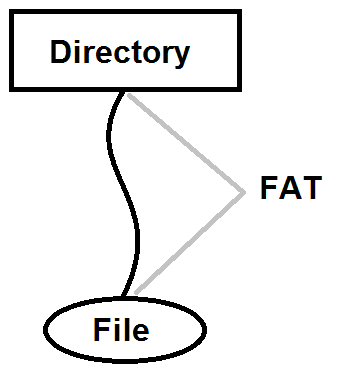
\includegraphics[width=0.4\textwidth]{fatgoed.png}
		\caption{Schematische weergave van de werking van een 	FAT}
		\end{center}
	\end{figure}

	\newpage
	\section{Fouten in de FAT}\label{sec:fout}
	\subsection{Fouten overzicht}\label{sec:overzicht}
	Er zijn verschillende soorten fouten die kunnen optreden in een FAT-12. Sommige fouten zijn eenvoudig op te lossen en op te sporen.\\\\
	Enkele fouten in de FAT die zijn op te sporen zijn bijvoorbeeld:
	\begin{itemize}
		\item Dubbel gebruik van een deel van de FAT
		\item Een file die twee keer voor komt in \'e\'en directory
		\item Geen overeenkomende langte in de directory en het aantal clusters
		\item Loops in de FAT
		\begin{itemize}
			\item Meerdere verwijzingen 
		\end{itemize}
		\item Incorrect eindigende link
		\item Een bestand dat bestaat in de directory maar niet in de FAT
	\end{itemize}
	Daarnaast zijn de volgende fouten niet op te sporen:
	\begin{itemize}
		\item Twee dezelfde files in verschillende directory's
		\item Een bestand komt nog voor in de FAT maar staat niet meer in de directory
	\end{itemize}

	\subsection{Dubbel gebruik van een deel van de FAT}\label{sec:dubbel}
	Een deel van de FAT mag niet dubbel gebruikt worden. Hiertoe wordt bijgehouden welke clusters al gelezen zijn. Wordt een cluster dubbel gelezen dan bestaat een file twee of meerdere malen. Of twee verschillende files die samen tot \'e\'en file mergen.

	\subsection{Geen overeenkomende lengte}\label{sec:lengte}
	De lengte van de file is bekend, echter kan het voorkomen dat deze lengte niet overenkomt met de FAT. Er treedt dan een fout op. De lengte in de FAT kan ofwel te lang ofwel te kort zijn. Is de lengte te lang dan is het aantal gelezen clusters groter dan het aantal clusters dat de file zou horen te hebben. Is de lengte te kort dan zijn er te weinig clusters gelezen dan zou moeten, de FAT denkt aan het einde te zijn terwijl dit niet zo is.

	\subsection{Loops}\label{sec:loops}
	In een FAT kunnen loops optreden. Er wordt dan een deel van de FAT meerdere malen aangeroepen. In een FAT mag dit niet voorkomen (zie \ref{sec:dubbel}). Om een loop op te sporen moet worden gekeken of een cluster dubbel gelezen wordt door \'e\'en file. Dit gebeurdt in dezelfde methode waarin al wordt gechecked of een file dubbel voorkomt. Wordt er een loop waargenomen dan moet deze worden verbroken, anders wordt er eeuwig doorgeloopd en wordt dezelfde foutmelding ook eeuwig gegeven.

	\subsection{Incorrecte links}\label{sec:links}
	Sommige links uit de FAT kunnen incorrect zijn. De aangegeven link behoord bijvoorbeeld niet bij de file in kwestie. Om deze foute links op te sporen worden FAT1 en FAT2 met elkaar vergeleken. Zijn ze niet aan hetzelfde dan is de link incorrect.\\
\LARGE \textbf{dit deel hierboven moet nog wat duidelijker }
\normalsize
	\subsection{Een bestand dat niet voorkomt in de FAT}\label{sec:dir}
	Het kan voorkomen dat een bestand niet (meer) bestaat in de FAT. 

	\section{Setup van het programma}\label{sec:setup}
	Om het programma te laten werken moeten alle files uit de gecomprimeerde map woorden gehaald en in een directory worden geplaatst. Vervolgens dient er via een commandshell genavigeerd te worden naar deze directory. Als de gebruiker in de juiste directory zit moet in de shell het commando 'make setup' worden uitgevoerd. 
Hiermee worden de juiste mappen aangemaakt die nodig zijn om de output in op te slaan. Als het eerste commando is uitgevoerd kan het volgende commando worden ingetypt. Dit is het commando 'make'. Alle code wordt nu gelinkt en gecompileerd tot twee werkende programma's: fat-checker \& fat-extracter. Zodra dit is gebeurd kunnen de programma's gebruikt worden. De meest eenvoudige manier om alle dick-images in \'e\'en keer uit te voeren en alle uitvoer weg te laten schrijven is door het commando 'make run' te gebruiken. Hierbij worden eerst alle files uit de disk-images weggeschreven door het programma fat-extract. De files worden per disk-image in de directory 'extract' opgeslagen. In de directory 'out' staan twee directorys, de uitvoer voor het wegschrijven van de files staat in de directory 'extracter'.
Vervolgens wordt het tweede programma, fat-checker, uitgevoerd. De uitvoer van dit programma wordt weggeschreven in de directory 'checker', de tweede directory in 'out'.
	
\end{document}
